% Derived sequences are saved separately from the accepted WT design.
\subsection{Sequence-Defined Control and Mutant Constructs}\label{sec:control-constructs}
Five plasmid conditions are defined: parental pEGFP-N1 expressing EGFP only, the accepted WT TFEB--EGFP reporter, and three derived reporters carrying S211A, S142A or S142A/S211A (Figures~\ref{fig:control-plasmids} and \ref{fig:mutant-plasmids}). Amino-acid positions refer to human NP\_009093.1. The fusion constructs share the same 6,134-bp plasmid architecture, the GDPPVAT junction and C-terminal EGFP, and encode 722 residues. The two single mutants and their combination allow site-specific and combined comparisons; they are not three interchangeable ``constitutively nuclear'' positive controls~\cite{Vega2017,Napolitano2018}.

\begin{table}[htbp]
\centering\small
\caption{Exact designed codon changes; plasmid coordinates are 1-based inclusive.}
\begin{tabularx}{\textwidth}{l l l Y}
\toprule Variant & Codon change & Plasmid nucleotides & Comparison enabled \\
\midrule
S142A & AGC $\rightarrow$ GCC & 1054--1056 & Recovery with or without the S142 phospho-acceptor \\
S211A & TCC $\rightarrow$ GCC & 1261--1263 & S211-dependent distribution and 14-3-3 association \\
S142A/S211A & Both changes & Both intervals & Combined perturbation versus each single mutant \\
\bottomrule
\end{tabularx}
\end{table}

Generate each mutant using a sequence-defined synthetic donor with the same cloning flanks as the accepted WT amplicon, followed by the established HindIII/BamHI workflow. The supplied donor FASTAs specify the intended DNA; they are not purchased or experimentally validated material. Existing cloning primers may amplify the matched donors, but new mutagenesis primers are not invented. Include no-template PCR, digested-vector-only ligation and the established positive transformation control for each batch. Sequence the full fusion region and both junctions in both directions, explicitly including both target codons. Use two independently recovered, sequence-correct bacterial clones per genotype for key-contrast confirmation to detect clone/preparation-specific effects; randomize clone identity across experimental days. Bacterial clones are not additional biological cell-culture replicates.

The derived sequences retain the WT reading frame and unique HindIII/BamHI cleavage geometry. Ordinary diagnostic band sizes therefore do not identify these point mutants; the existing gel predictions apply to their gross insert/backbone sizes only. Sequence acceptance, intact expression and cell phenotype are three distinct checks. Alanine removes the serine phospho-acceptor but can also alter local interactions; none of these substitutions alone proves the responsible kinase or a direct phosphorylation reaction. A phosphomimetic S-to-D/E construct is not included as a guaranteed phosphorylated-state control.

\begin{figure}[htbp]
\centering
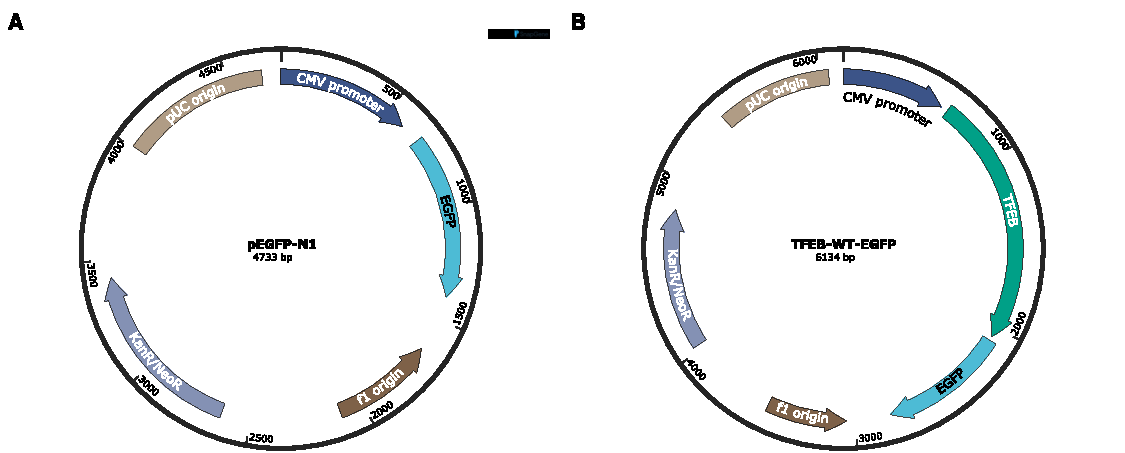
\includegraphics[width=\textwidth]{images/B/control-plasmids.pdf}
\caption{SnapGene Viewer maps of (A) the 4,733-bp EGFP-only control and (B) the 6,134-bp WT TFEB--EGFP reporter. Selected features retain their sequence coordinates and use a consistent NPG palette. The linker and minor regulatory annotations are omitted at this scale; complete GenBank records accompany the design. Native SVG geometry and vendor credit are preserved; the size unit is typeset in English. These are designed constructs, not verified experimental clones.}
\label{fig:control-plasmids}
\end{figure}

\begin{figure}[htbp]
\centering
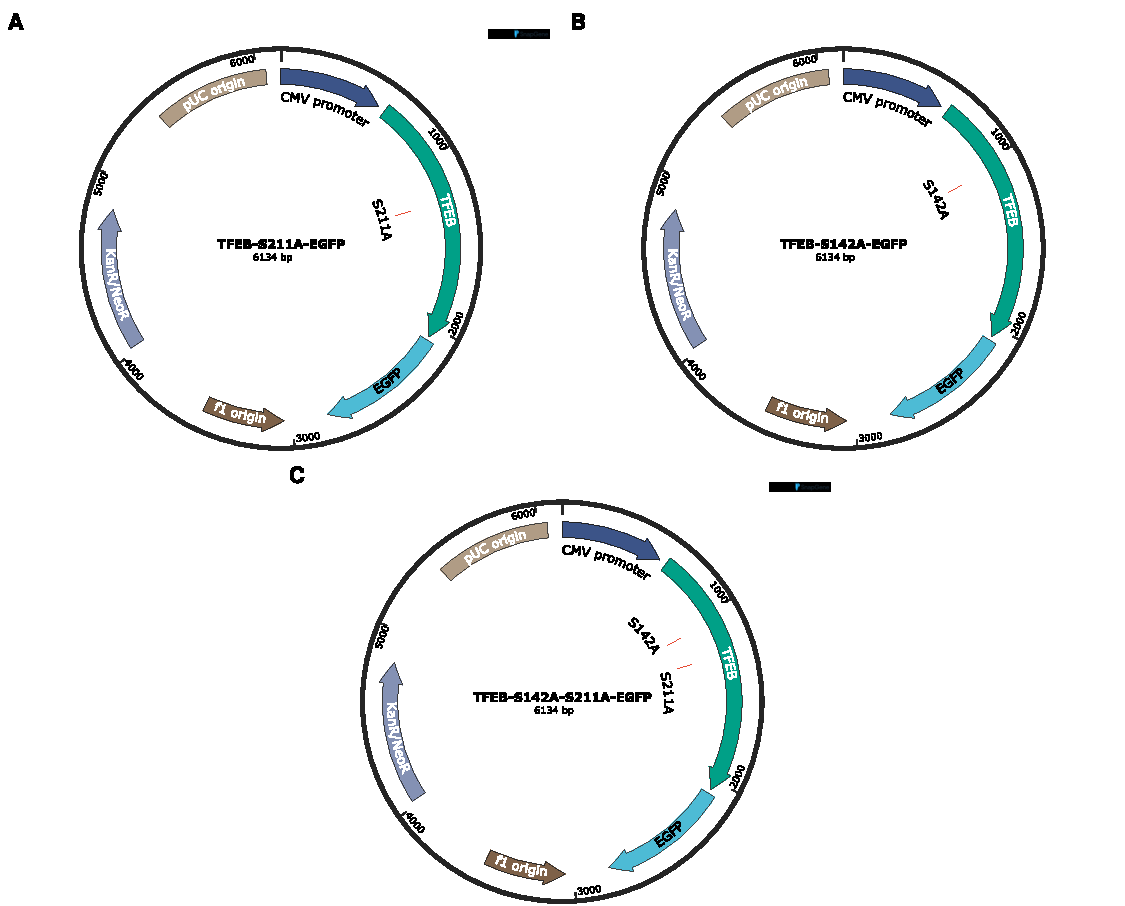
\includegraphics[width=0.98\textwidth,height=0.74\textheight,keepaspectratio]{images/B/mutant-plasmids.pdf}
\caption{SnapGene Viewer maps of (A) S211A, (B) S142A and (C) S142A/S211A. Red marks identify the substituted codons; residue numbering refers to NP\_009093.1. Every plasmid remains 6,134 bp and encodes 722 residues. EGFP, backbone and linker sequences remain identical to WT. These substitutions define experimental comparisons and do not establish a constitutively nuclear phenotype.}
\label{fig:mutant-plasmids}
\end{figure}
\FloatBarrier
